% -----------------------------------------------
% Template for ICMC SMC 2014
% adapted and corrected from the template for SMC 2013,  which was adapted from that of  SMC 2012, which was adapted from that of SMC 2011
% -----------------------------------------------

\documentclass{article}
\usepackage{icmcsmc2014}
\usepackage[]{biblatex}
\addbibresource{SpatDIF.bib}
\usepackage{times}
\usepackage{ifpdf}
\usepackage[english]{babel}
\usepackage{listings}
\usepackage{enumitem}
\usepackage[export]{adjustbox}
\sloppy
\setlist[itemize]{itemsep=0.0pt, topsep=1.5pt}

%user defined variables
\def\papertitle{The SpatDIF library - Concepts and Practical Applications in Audio Software}
\def\firstauthor{Jan C. Schacher}
\def\secondauthor{Chikashi Miyama}
\def\thirdauthor{Trond Lossius}

% pdf-tex settings: detect automatically if run by latex or pdflatex
\newif\ifpdf
\ifx\pdfoutput\relax
\else
   \ifcase\pdfoutput
      \pdffalse
   \else
      \pdftrue
\fi

% \ifpdf % compiling with pdflatex
  \usepackage[pdftex,
    pdftitle={\papertitle},
    pdfauthor={\firstauthor, \secondauthor, \thirdauthor},
    bookmarksnumbered, % use section numbers with bookmarks
    pdfstartview=XYZ % start with zoom=100% instead of full screen; 
                     % especially useful if working with a big screen :-)
   ]{hyperref}
  \pdfcompresslevel=9

  % \usepackage[pdftex]{graphicx}
  \usepackage{graphicx}
  \usepackage[export]{adjustbox}
  \DeclareGraphicsExtensions{.pdf,.jpeg,.png}

  \usepackage[figure,table]{hypcap}
	
% \else % compiling with latex
%   \usepackage[dvips,
%     bookmarksnumbered, % use section numbers with bookmarks
%     pdfstartview=XYZ % start with zoom=100% instead of full screen
%   ]{hyperref}  % hyperrefs are active in the pdf file after conversion
% 
%   \usepackage[dvips]{epsfig,graphicx}
%   % declare the path(s) where your graphic files are and their extensions so 
%   %you won't have to specify these with every instance of \includegraphics
%   \graphicspath{./figures/}
%   % \DeclareGraphicsExtensions{.eps}
% 
%   \usepackage[figure,table]{hypcap}
% \fi

%setup the hyperref package - make the links black without a surrounding frame
\hypersetup{
    colorlinks,%
    citecolor=black,%
    filecolor=black,%
    linkcolor=black,%
    urlcolor=black
}

\title{\papertitle}

% Authors
% Please note that submissions are NOT anonymous, therefore 
% authors' names have to be VISIBLE in your manuscript. 

 \threeauthors
   {\firstauthor} {Zurich University of the Arts\\
   Institute for Computer Music\\ and Sound Technology ICST\\
     {\tt \href{jan.schacher@zhdk.ch}{jan.schacher@zhdk.ch}}}
   {\secondauthor} {University of Music, Cologne\\ 
   Studio for Electronic Music\\
     {\tt \href{me@chikashi.net}{me@chikashi.net}}}
   {\thirdauthor} { Bergen Center for Electronic Arts BEK\\ %
     {\tt \href{trond.lossius@bek.no}{trond.lossius@bek.no} }
}

\begin{document}

\capstartfalse
\maketitle
\capstarttrue

\begin{abstract}
The development of the Spatial Sound Description Interchange Format SpatDIF continues with the implementation of concrete software tools.
In order to make SpatDIF usable in audio workflows, two types of code implementations are developed.
The first is a C/C++ software library called `libspatdif', whose purpose is to provide a reference implementation of SpatDIF.
We show the class structure of this library and discuss its main components and how they embody the principles derived from the concepts and specifications of SpatDIF.
The second type of tool are specific implementations in audio programming environments, which demonstrate the methods and best-use practices for working with SpatDIF.
Two practical scenarios are shown in functional examples, demonstrating the use of externals in MaxMSP and Pure Data as well as the implementation of the same example in C++ .
Finally, the article addresses the possible evolution of the syntax and further development of the software system for spatial sound description.

\end{abstract}

\section{Background}\label{sec:background}

The Spatial Sound Description Interchange Format SpatDIF presents a structured syntax for describing spatial audio information, addressing the different tasks involved in creating and performing spatial sound scenes.
The goal of this approach is to simplify and enhance the methods of creating spatial sound content and to enable the exchange of between otherwise incompatible software. 
SpatDIF proposes a simple and extensible format as well as best-practice examples for storing and transmitting spatial sound scenes. 
It encourages portability and the exchange of compositions between venues with different surround audio infrastructures. 
SpatDIF also fosters collaboration between artists such as composers, musicians, sound installation artists as well as researchers in the fields of acoustics, musicology, and sound engineering.
SpatDIF was developed in a collaborative effort and has evolved over a number of years.

The community pages as well as all the related information and publications can be found at \href{http://www.spatdif.org}{www.spatdif.org}.\footnote{All URIs in this article were last accessed in April 2014.}

% \subsection{Project History}\label{subsec:project_history}

SpatDIF was coined in \citeyear{peters_caa07} \cite{peters_caa07} when Peters posited the need for a format describing spatial sound scenes in a structured way, since at that time all of the available spatial rendering systems used self-contained, proprietary syntax- and data-formats.
Through a panel discussion \cite{2008ICMCpanel, Peters:2008spatdif} and other meetings and workshops, the scope and concepts of SpatDIF were extended, refined, and consolidated.
After an extended process the SpatDIF specification was informally presented to the spatial sound community at the ICMC in Huddersfield in August 2011 and at a workshop at the TU-Berlin in September 2011.
The responses in these meetings suggested the urgent need for a lightweight and easy to implement spatial sound scene standard, which would contrast the complex MPEG-4 scene description specification \cite{scheirer1999audiobifs}.

The completion of a first usable version of the specifications \cite{SpatDIF_03} defining the core descriptors and a few indispensable additional descriptors was achieved the following year. The publication of this project milestone at the SMC in Copenhagen \cite{SpatDIF_SMC12} won a best paper award and was subsequently published in the Computer Music Journal \cite{Peters:2013SpatDifCMJ}.
This encouragement incited the group to tackle the task of proving that the concept would work in actual software.

% \subsection{Design Principles}\label{subsec:design_principles}

A central principle for SpatDIF is the conceptual separation of authoring and rendering of spatial sound scenes or pieces. They may occur at separate times using the same or differing infrastructure, at separate places either simultaneously or with a long time between the two and of course through a mixture of these factors. 
The exact modality should not have to be determined at the outset.

In addition to the separation of the basic functionalities two principal use-cases can be distinguished.
The first scenario is focused on storing spatial audio pieces on a support for future playback. 
The second scenario deals with streamed content and scene information in real- or near real-time.
For these applications SpatDIF formulates a concise semantic structure that is capable of carrying all the information relevant for preserving a sound scene, without being tied to a specific implementation or technical method.
Since SpatDIF is a syntax rather than a programming interface or file-format it may be represented in any of the current or future structured mark-up languages or messaging systems.
It describes only those aspects required for the storage and transmission of \emph{spatial sound information}.
Because a complete work typically contains aspects that are outside the realm of spatial sound scenes, SpatDIF provides descriptors to link these aspects to the spatial dimensions, but only to the extent necessary.
% For example, the description of media-streams in SpatDIF is necessary in order to define the storage location or origin of the audio present in the scene.
% For example, to be able to render the audio objects with the correct audio content in the spatial scene, the storage location of the audio content needs to be defined via SpatDIF's media resources.
For example, the description of media-streams in the Media extension is necessary in order to describe from where the sounding content of the scene originates.

\section{Library Concepts}\label{sec:libspatdif_concepts}

In this article we present the development and implementation of software tools aimed at easy integration of SpatDIF into existing software and workflows.
The concepts and guidelines laid down in the SpatDIF specifications are implemented in a software-library.
In addition to the low-level library to demonstrate the utlisation of SpatDIF, example applications which utilise this library were created and will be discussed below.
The use of this library is demonstrated in externals for MaxMSP\footnote{\href{http://www.cycling74.com}{www.cycling74.com}} and PureData \footnote{\href{http://puredata.info}{puredata.info}} as well as in an application written entirely in C++ in the creative coding environment OpenFrameworks.\footnote{\href{http://www.openframeworks.cc}{www.openframeworks.cc}}

After establishing a coherent specification with example use-cases in textual form only, the next development step is the implementation of software, which embodies the specified concepts and should serve as a reference for future work.
For this purpose a platform-independent software library written in C/C++ was designed and is now implemented. \cite{Miyama_2013}
By providing a software library rather than just a complete software application, implementations in many different software environments are facilitated, which is one of the goals of the project.
The library is in charge of holding one or more spatial audio scenes and provide ways to read and write elements to and from this scenes, either directly from native code or via OSC-formatted messages, that may originate from within the application or or come in from an external source via the network.

\subsection{Separation between Library and Client}\label{subsec:separation}

The separation of tasks between the library and a client application is deliberate.

On the one hand, it is the library that builds and maintains in memory the SpatDIF scene, either obtained from an already existing description stored in a file, or on-the-fly in real time from elements received via OSC-formatted messages.
It provides an application programming interface (API) that hides most of the complexity of handling the scene data.

The client application, on the other hand, is in charge of loading the file containing the SpatDIF-scene from the file system and handing it to the library in a text buffer.
In addition, the client application open network sockets and forwards OSC-formatted data to the library.
It queries the library for scene information at initialisation as well as at runtime, based on its own scheduler, thereby actively playing the scene.
The client application also deals with all the audio related processes, such as loading audio files, playing them back, configuring the audio-system and spatialising the audio to generate a surround audio experience.
Information necessary to achieve this is provided by the SpatDIF scene, but it is beyond the scope of SpatDIF to cover the specific details of all possible surround audio configurations.
More details are discussed below in the sections describing the specific software tools.


\begin{figure}[h]
	\centering
	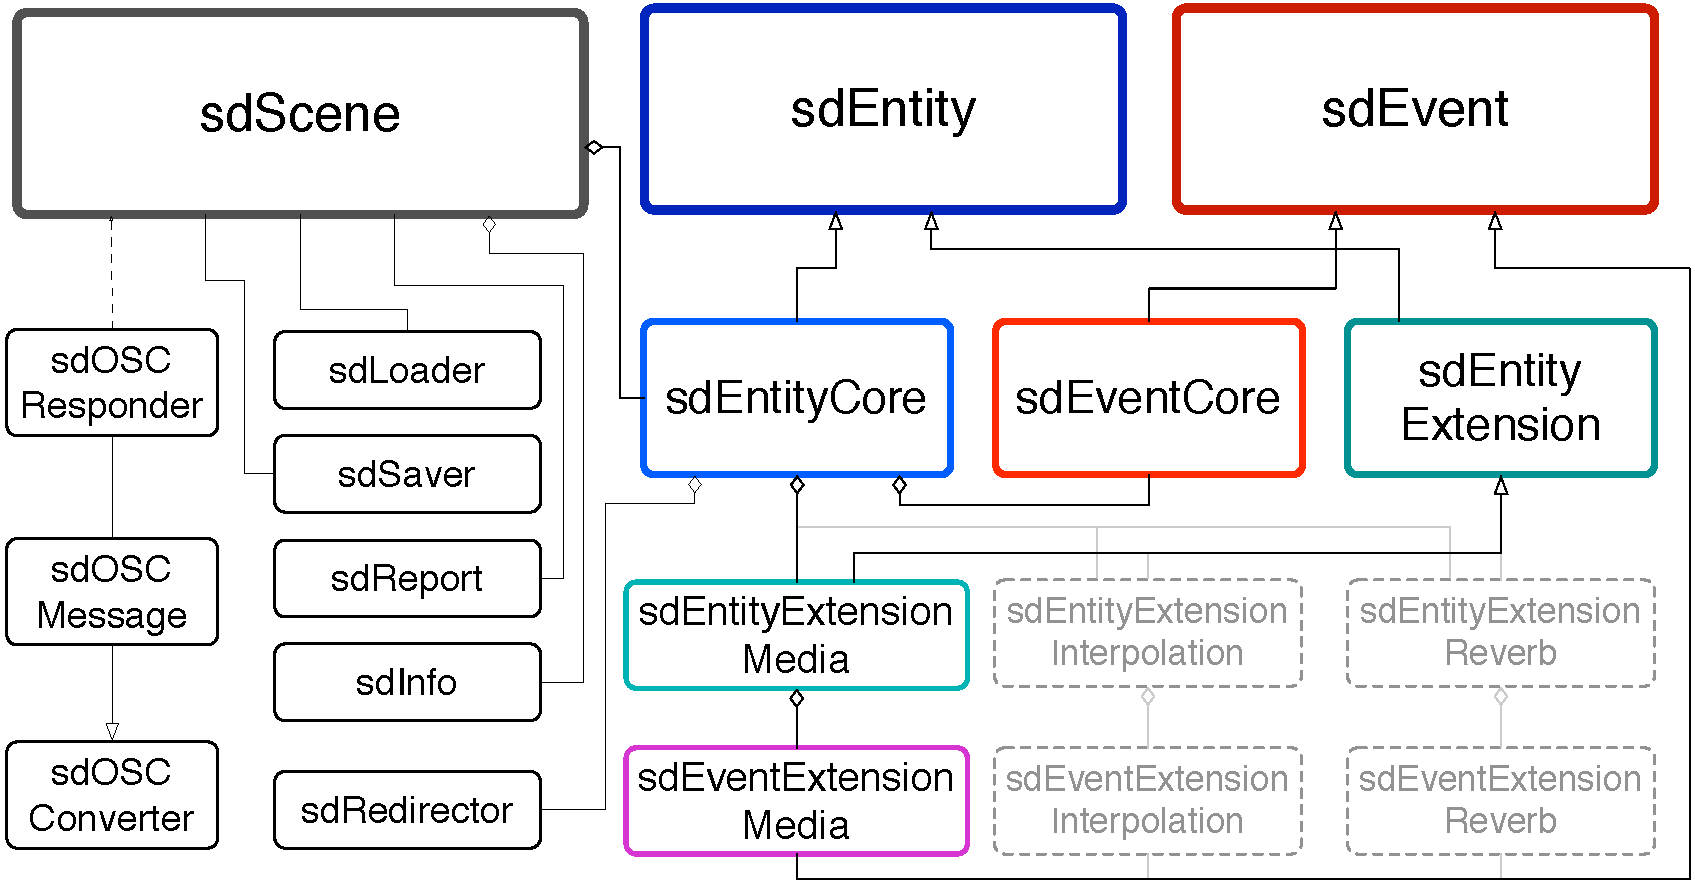
\includegraphics[width=0.95\columnwidth]{class_diagram.pdf}
	\caption{Simplified class hierarchy of the SpatDIF software library.
	\label{fig:class_structure}
}
\end{figure}

\subsection{Library Class Structure}\label{subsec:class_structure}

The class hierarchy described here is intended to show the relationship between the scene and its contents, as well as their hierarchical dependencies (see Figure \ref{fig:class_structure}). 
An instance of \emph{sdScene} class represents a SpatDIF scene and maintains instances of \emph{sdEntityCore}. The functionalities of \emph{sdEntityCore} may be extended by the descendants of \emph{sdEntityExtension}. 
The activation and deactivation of the extension are global within a scene, therefore \emph{sdScene} is also responsible for the extension handling.
Each instance of \emph{sdEntityCore} maintains instances of \emph{sdEvent}, which represent events of the entity they are attached to.

The following are brief descriptions of the most important classes.

\begin{itemize}[leftmargin=-0.0mm]
\item[] \emph{sdScene}\\
An instance of \emph{sdScene} maintains all data associated to a SpatDIF scene. This class offers clients the following three main functionalities: Addition, deletion and modification of \textbf{entities} in the scene; Addition and modification of the \textbf{meta data} associated to the scene; Activation and deactivation of the \textbf{extensions} in the scene.

Once the client activates an extension in a scene, \emph{sdScene} automatically adds extended functionalities and allocates extra buffers to all existing and newly created instances of \emph{sdEntityCore}. 
Symmetrically, when deactivating an extension, \emph{sdScene} removes all extended functionalities and previously allocated buffers from all existing \emph{sdEntitieCores}, leading to the deletion of all data stored in the extension buffers.

\item[] \emph{sdEvent}\\
This is a pure abstract class of event, that maintains the following three data items: \textbf{time} - absolute time of the event; \textbf{descriptor} - type of event; \textbf{value} - actual data.

\item[] \emph{sdEntity}\\
This is a pure abstract class of entity in SpatDIF scenes. Basic functionalities, such as addition, deletion, and modification of events are implemented.

\item[] \emph{sdEntityCore}\\
An instance of \emph{sdEntityCore} maintains events with SpatDIF core descriptors and a vector storing instances of SpatDIF extensions. 
This class replies to queries from the client about events, e.g. if a client asks a \emph{sdEntityCore} a value of a certain descriptor at a specific time, the \emph{sdEntityCore} returns the value. 
The client is able to raise an query about multiple events within a certain time frame and filter events by descriptors. 

\item[] \emph{sdEntityExtension}\\
This is a pure abstract class of extensions. The descendants of this class. e.g. \emph{sdEntityExtensionMedia} handles the events with extended descriptors. 
If a client activates an extension in a scene, each existing instance of \emph{sdEntityCore} instantiates the designated subclass of \emph{sdEntityExtension} and register it in its internal vector.

\item[] \emph{sdLoader/sdSaver}\\
These two classes provide several utility functions and enable clients to create an instance of \emph{sdScene} from a XML, JSON, or YAML string and vice versa. 
In order to maintain platform independence and to achieve maximum flexibility, the library does not handle files directly, the client software is responsible for the file management. 
These functions use two external libraries for parsing of markup formatted strings: TinyXML-2\footnote{\href{http://www.grinninglizard.com/tinyxml}{www.grinninglizard.com/tinyxml} } and libjson\footnote{\href{http://sourceforge.net/projects/libjson}{sourceforge.net/projects/libjson} }.
\end{itemize}

% TODO @Trond/Chikashi decide if the code-examples should stay in this paper, since this paper is mainly about the externals an should be different enough from the JSSA paper from last december. Perhaps an extract from the turena's file would be more appropriate here? [jasch]
% \subsection{Simple Code Example}
% The following code listing shows the native C++ calls used to load an XML-formatted string obtained from a SpatDIF file into an \emph{sdScene} and query the entity called `insect' for the first occurrence of an event which contains a position and a media descriptor.
% 
% \lstinputlisting[columns=fullflexible, breaklines=true, numbers=left,xleftmargin=3.0em,frame=none,framexleftmargin=0.0em, basicstyle=\scriptsize\ttfamily]{example_code2.cpp} 
% 
% \noindent The code produces this console-output: 
% \lstinputlisting[columns=fullflexible,breaklines=true,numbers=none,xleftmargin=1.0em, basicstyle=\scriptsize\ttfamily]{code_output.txt} 
% 
% \noindent 
% The following processes are executed in the example:
% 
% \noindent Line 1: the \emph{sdLoader::sceneFromXML} function loads a scene from an XML formatted string.
% 
% \noindent Line 2: A pointer to an entity named `insect' is obtained by the \emph{scene.getEntity} function.
% 
% \noindent Lines 3 -- 4: Entity `insect' is requested for the first event with position and media location descriptor.
% 
% \noindent Line 5: Query `insect' entity for its name.
% 
% \noindent Lines 6 -- 8: Post values and time of events.

\subsection{Example Scene}\label{example_scene}

The canonical piece `Turenas' by John Chowning (see also \cite{Peters:2013SpatDifCMJ}), serves as test-case in the following examples. 
The beginning of the SpatDIF file, including only the `insect' trajectory at second 0:44, contains the following elements in an XML format:

\lstinputlisting[tabsize=3,columns=fullflexible,breaklines=true,numbers=none,language=XML,morekeywords={source,sink,time,meta},basicstyle=\scriptsize\ttfamily]{turenas_insect_example.xml} 

The corresponding sound files have to be stored and transported alongside the SpatDFI file proper. 
It is therefore important to think in terms of ‘SpatDIF bundles’ or projects rather than single files. 
However, it was a deliberate choice not to propose a format that combines sound-files and scene descriptors in a binary format, since human-readability without additional software tools would be lost.

\section{Introducing the SpatDIF Externals}\label{sec:Intro}

The SpatDIF syntax is an implementation-independent specification, rather than a specific software interface. 
However, the actual value of using it only becomes evident in real applications. 
Although SpatDIF was developed with a number of different scenarios in mind, the use-case most closely associated with the authors' practices are electro-acoustic surround audio compositions for concerts and installations or real-time spatialisation in computer music performance.
Therefore, the first code implementations of the SpatDIF library are made with tools for real-time audio software.

\subsection{Practical Application}\label{practical_usage}

In order to explore the methods and actual handling of the `libspatdif' in a real situation, a dual testbed was implemented as externals for MaxMSP and Pure Data.
Apart from small differences in the two environments, mainly concerning the handling of files, the two implementations are identical.
In addition, an example application with a limited feature-set was written in openFrameworks, mainly to establish and test a workflow done entirely in the C++ language.

There are a number of concepts that need to be taken into account when using the library, which inform the design of the implementations shown here.

The library serves as a data-storage for audio scenes that needs to be queried for its information in specific ways.
It doesn't provide a scheduling mechanism of its own, rather, the client application is responsible for executing all time-related functions.
This design choice is explicitly geared towards temporal flexibility, i.e. slowing down or speeding up playback, jumping an cueing, which are features that can only properly be implemented by the end-user.

There are two main interfaces for the library, the native call and the OSC-command.
The native commands call functions of the library within C/C++ code whereas the OSC-commands get handed to the library as messages conforming to the OSC syntax.
The library doesn't implement network socket handling functionalities, this is the client environment's task.
In order to input and output information directly to/from the scene, the name-space is described with hierarchical addresses that have to conform to the SpatDIF specification.
In the implementation of the externals, the input of elements into the scene stays in the OSC-style with a slash delimited format, whereas in the output from the scene the addresses are converted to a space-delimited format to avoid a dependency on an additional OSC-parser.

Additional commands that are directly addressing functions of the library have a different syntax, which is not part of the SpatDIF specifications, but rather specific to the implementation of the library.
These \emph{/spatdifcmd} messages concern the querying of information from the library and the setting and getting of variables necessary for the executing the queries.

File operations are not functions of the library itself.
The externals in MaxMSP and PureData implement the required file loading and saving methods, which are specific to their own environment. 
 % TODO: maybe a switch could be implemented to change this behavior back and forth?
 
\begin{figure}[httb]
	\centering
	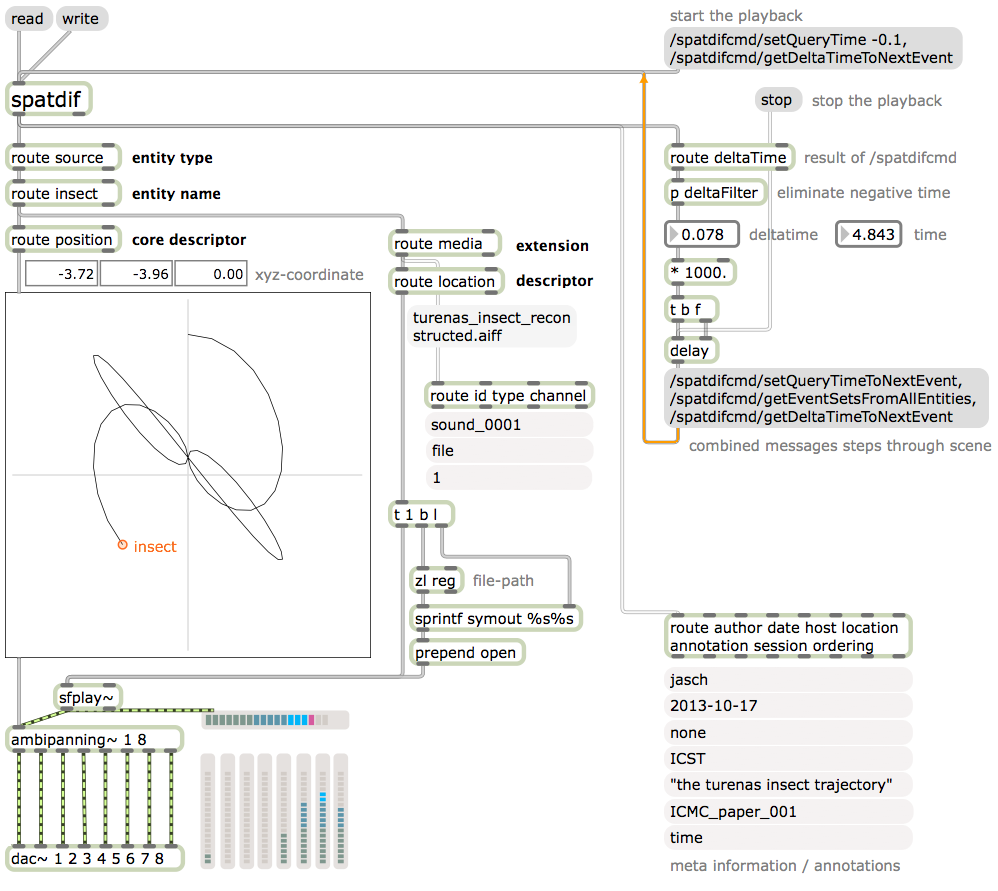
\includegraphics[width=\columnwidth]{playback_maxpatch.png}
	\caption{Implementation of SpatDIF in a MaxMSP external, demonstrating the playback of the Lissajous trajectory from Chowning's `Turenas'.} 
	\label{fig:screenshot}
\end{figure}

\subsection{Playback}\label{subsec:playback}

The first example shown here centres around file-handling and the playback of a SpatDIF scene in a multichannel setup.
Figure \ref{fig:screenshot} shows this with a simplified monophonic setup in MaxMSP.
This workflow makes a few assumptions which are not limitations of libspatdif as such, but help to clarify the concepts.
The program demonstrates the rendering of an existing scene, which in this instance is the `insect' trajectory from John Chowning's ``Turenas'' (1972) \cite{chowningturenas}.
The scene is stored on disk in a SpatDIF-formatted XML-file together with the audio content as sound-file.
After reading the scene from disk, the meta section can be parsed to obtain annotation information, as shown in the lower right.

In a fully dynamic system, additional information is required to set up the rendering algorithm.
For this purpose queries are made to the library to obtain information about the number of entities present in the scene and the names of the entities as well as the extensions that are present.\footnote{For more specific information about the concept of extensions in SpatDIF, please refer to \cite{SpatDIF_SMC12, Peters:2013SpatDifCMJ, SpatDIF_03}. }
This allows to determine the number of playback voices needed and then to set up the hierarchical message routing according to the names of entities.
In this example this step is omitted and only one playback voice is implemented with a hard-coded message-routing set to the entity-type of \emph{source} and the entity-name called \emph{insect}.
Subsequently, the messages are routed to obtain the \emph{position} core-descriptor required for the spatialisation process as well as the \emph{media} extension with the \emph{location} descriptor necessary to load files for playback.
The sound-file player, visualisation \cite{Schacher_ICMC_2006} and spatialisation algorithms shown here represent the minimal case and of course would normally be more fully implemented. %\cite{schacher7Years}

As mentioned earlier the library does not have its own scheduling mechanism. 
In this example this becomes apparent and therefore the method for time-based playback is demonstrated.
In the right half of the example are shown the \emph{spatdifcmds} necessary to run iteratively through the scene.
The basic action is to ask with \emph{getDeltaTimeToNextEvent} for the delta times between subsequent events.
Since a scene can contain sparse data at no fixed intervals, it is crucial to have a dynamic timing mechanism for playback.
The command \emph{setQueryTimeToNextEvent} sets the query time variable to the next event, then the library gets queried for all the events at that point in time with \emph{getEventSetsFromAllEntities}, and finally the time to wait until the next event is queried again.
These commands form a loop that steps through the scene, which is rendered visible in the figure through the orange connection flowing back to the spatdif-external.
The timing is executed by a delay which waits the appropriate amount of time to the next event before re-triggering the same sequence.
These commands are global to the scene, so that all events associated with any entity in the scene are retrieved.
If only events from selected entities are desired, this can be achieved by filtering in the message routing system, or as will be shown below with more specific commands to the library. %TODO find out if we we provide other interface calls to the library across the OSC-cmd interface.



\subsection{Recording}\label{subsec:recording}

In the second example shown in Figure \ref{fig:screenshot2}, spatialisation information originating from real-time input via a physical controller is recorded into a SpatDIF scene.
Four joysticks are set up to control the playback and spatialisation of four monophonic point-source entities in a scene.
As in the previous case, this example is a simplification of a real application, yet still represents a fully functional implementation.
The patch is divided into two processes that run in parallel, the recording on the right side depending on the
realtime processing on the left.
 
In the left half of the Figure \ref{fig:screenshot2}, the real-time process starts from the controller-input and leads to sound spatialisation and multichannel output.
The controller-input at the top feeds into a visualisation-tool before reaching directly the spatialisation-module.
Underneath, keyboard-commanded start/stop switches and file-selection menus control four sound-file playback modules.

On the right hand side of Figure \ref{fig:screenshot2} are the parts necessary to record the key-events into a SpatDIF-scene.
The large message-box in the right shows the initialisations necessary to set up the scene.

In this example, each voice independently activates the recording of position information in synchrony with its file-playback.
This mechanism is shown in the `p voice' sub-window. 
Here, the \emph{setPosition} spatdif commamd is formatted with the correct entity-name and combined with the real-time position data arriving from the visualisation tool.
Further spatdif commands to set media events are \emph{/media/setType} and \emph{/media/setLocation}.
They are tied to specific entities, and therefore need to be formatted with the entity-name and combined with the file-type and file-path of the media resources.

\begin{figure}[httb]
	\centering
	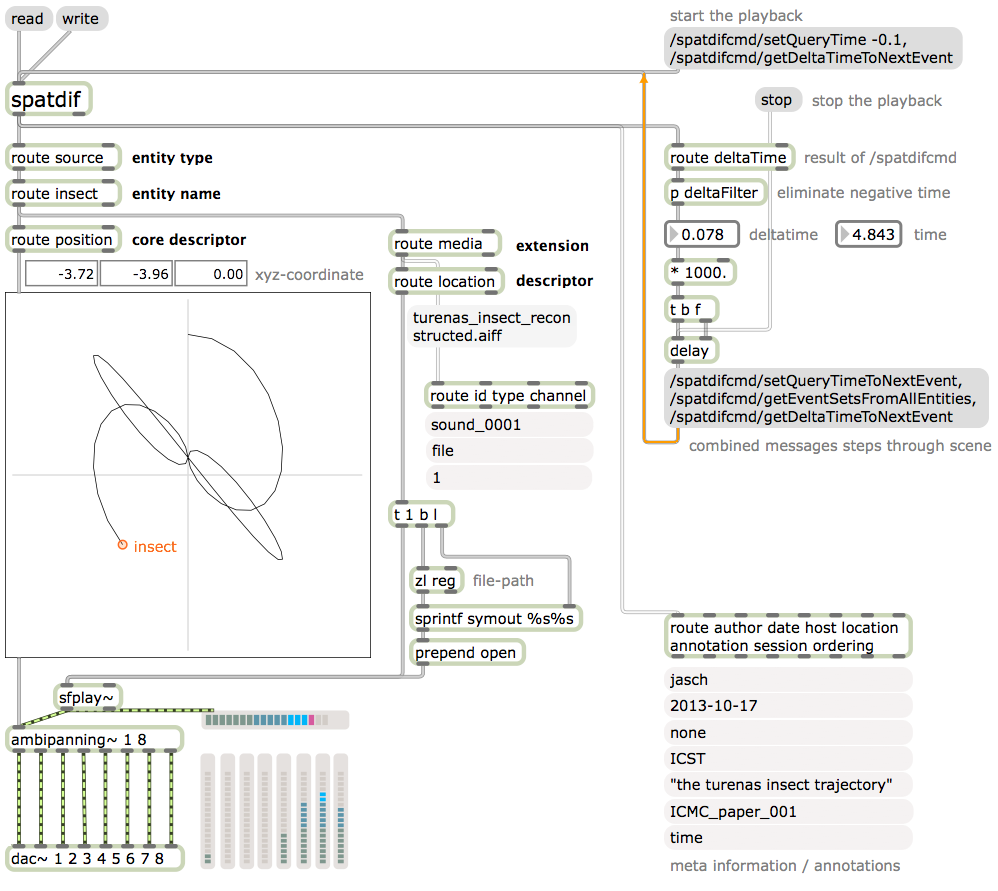
\includegraphics[width=\columnwidth]{recording_maxpatch.png}
	\caption{MaxMSP implementation, demonstrating the recording of four manually generated trajectories obtained from joysticks. The upper right shows the `voice' section responsible for formatting the media and position inputs.} 
	\label{fig:screenshot2}
\end{figure}

Once the media- and position-commands are formatted, they are sent directly to the spatdif-external for storage under a time-stamp obtained from the system.
This time-stamp is calculated as relative time since the beginning of the recording and is represented in seconds, formatted as doubles, i.e. 64-bit floating point values.

The \emph{setWriteTime} commands sets the writing `cursor' in the scene, which will apply to all messages that arrive until a new value for the `writeTime' variable is set.
Grouping all incoming events in this way may be regarded as a type of `frame-based' time-stamping and is defined in the SpatDIF-specification as a scene ordering according to time.

A `track-based' ordering of the events is also possible with this method, as is demonstrated in this example.
All events belonging to each entity may be recorded separately, and their time can be reset by setting the `writeTime' variable to zero when starting the recording of a new entity's events.
This `overdubbing' method works without problems when different entities are concerned (entities here are synonymous for voices or tracks).
When overdubbing events of the same entity, however, is it only possible to directly overwrite events if the time-stamps correspond exactly to the ones already stored, as could be the case for example for points in time generated by an algorithmic processes. 
In a real-time case this is difficult, if not impossible, to guarantee, therefore it is advisable to clear an entity's entire content with a call to the commands \emph{/removeEntity} followed by \emph{/addEntity} before re-recording events.

In general, all interaction with `libspatdif' occurs through the \emph{spatdifcmds}-syntax.
In a future version, input of pure SpatDIF-formatted OSC-messages will be implemented, eliminating the need to reformat the information to the \emph{spatdifcmd} syntax.




\section{Implementation in C++}\label{subsec:code_application}

The C++ example application implements the entire workflow for the playback of a SpatDIF scene. 
The application is called a `renderer' in analogy to visual tools, because it renders audible, in a surround setup, the information contained in a SpatDIF `bundle'.

The implementation has to solve all the question relating to file-handling, handling OSC-streams, instantiating the voices of the playback engine, panning, distance cues, and handling other descriptors present in the SpatDIF specifications version 0.3, (see \cite{SpatDIF_03}.
% 
% \subsection{Scope}

In order to provide a relevant example for the application of the `libspatdif', the scope of the application has been limited deliberately.
The panning algorithm is a simple spatial windowing algorithms named ``ambipanning'' \cite{Neukom:2008ambipan} that is highly flexible, easy to implement, not tied to a specific number of speakers and usable without modification both in two and three dimensional spatialisation situations.
The application provides a stand-alone implementation, with a basic 3D visualisation of the scene, and the possibility to play the scene in a stereo speaker setup.
It allows to load a SpatDIF file with associated sound files and play it through a few predefined multichannel speaker layouts.



This application is implemented in OpenFrameworks, which provides a powerful C++ toolset and a thriving community.
It provides both a sonic and visual rendering of the scene.
In analogy to the externals for MaxMSP and Pure Data, this implementation encapsulates all the functionalities concerning calls to the library in it own class named `ofxSpatDIF'.
This `addon' reflects the interface found in the externals.
Since OpenFrameworks is not particularly oriented towards audio, the classes provided for sound processing are somewhat rudimentary.
However -- and that is its strength -- many extensions exist and it is simple to add new functionalities and tie in external libraries.
`libsndfile'\footnote{\url{http://www.mega-nerd.com/libsndfile}} is such an external library. 
It provides a powerful audio file handling toolset and is linked in as a dynamic library, as is stipulated by its license.

The visual representation is a bare-bones wireframe drawing of the scene in OpenGL.
Figure \ref{fig:screenshot3} shows the scene of the example application.
The sound playback is processed through the sound-stream interface provided by the environment.
The process is straightforward, even if its implementation is a bit delicate.
After retrieving samples from the sound files via `libsndfile', panning and distance correction is applied to the signals, before the blocks of audio-samples are output.
The signal processing chain is deliberately kept simple, to provide a clear example of the implementation of such a process.


\begin{figure}[httb]
	\centering
	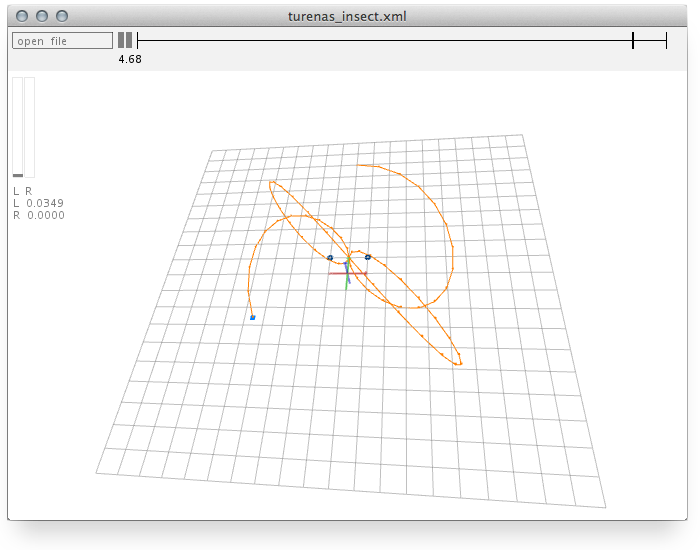
\includegraphics[width=\columnwidth]{of_screenshot.png}
	\caption{OpenFrameworks implementation of SpatDIF, demonstrating again the playback of the `insect' trajectory from `Turenas'} 
	\label{fig:screenshot3}
\end{figure}


\section{Conclusions and Future work}\label{sec:conclusions_future_work}

In this article we have shown concrete implementations of the Spatial Sound Description Interchange Format in software.
The examples presented here show limited use-cases, which need to be worked out more fully in a real-life applications.
The intention is to provide a simple method for working with SpatDIF in audio coding environments that is flexible enough to handle all layers of a spatial audio workflow. \cite{PetersSMC09}
A greater challenge is the application of these tools in commercial hosts, in particular DAWs that only expose a small part of their structure, for example to the access by plug-ins.

A short-term goal of this project is the complete implementation of the SpatDIF specifications version 0.3 \cite{SpatDIF_03} within the C++ library.
In addition, the methods for purely OSC-driven input and output have to be completed as well as loading and saving of scenes in other markup languages such as JSON.

In a wider perspective, the definitions of further extensions, as laid out in the current specifications, will increase the utility of SpatDIF.
In addition, the introduction of new entities, for example of `room' type should enable the description of room acoustics in the reverb extension.
The next round of specifications will build on the experience gathered while implementing SpatDIF in the code shown here and will take less effort to integrate into the library, externals and addons thanks to its consistent and open design.

%The limited space of this article prevents us from providing full code examples, but 
The externals, their source code and the C++ implementation are open-source and may be obtained via git from:\\ \footnotesize\url{http://code.zhdk.ch/git/spatdifrenderer.git}.\normalsize

% \vspace{0.5cm}

\begin{acknowledgments}
This development is funded by the Institute for Computer Music and Sound Technology of the Zurich University of the Arts.
\end{acknowledgments} 

\printbibliography

\end{document}
